% !TeX root = ../main.tex
% @file mainmatter/03_method.tex
% @brief Chapter 3: 手法

\chapter{手法}

\section{数式の例}

基本的な数式の例を示す．

\begin{equation}
    E = mc^2
\end{equation}

複数行の数式は次のように記述できる．

\begin{align}
    a + b & = c \\
    d + e & = f
\end{align}

行列の例を示す．

\begin{equation}
    A =
    \begin{bmatrix}
        1 & 2 \\
        3 & 4
    \end{bmatrix}
\end{equation}

\section{図の例}

図\ref{fig:example}に図の例を示す．

\begin{figure}[H]
    \centering
    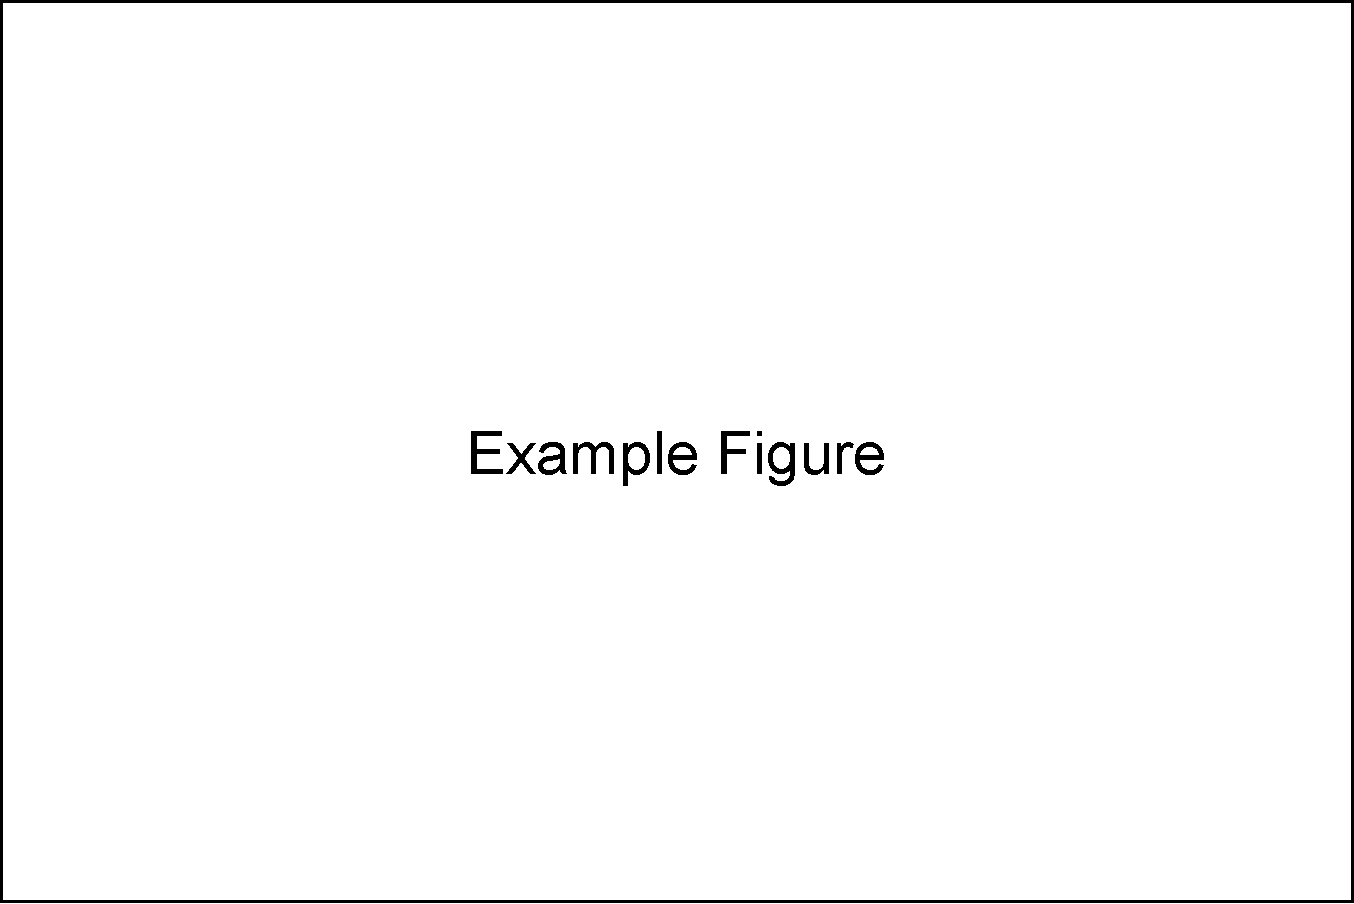
\includegraphics[width=0.5\linewidth]{figures/example.pdf}
    \caption{図の例}
    \label{fig:example}
\end{figure}

\section{表の例}

表\ref{tab:example}に表の例を示す．

\begin{table}[H]
    \centering
    \caption{表の例}
    \label{tab:example}
    \begin{tabular}{ccc}
        \toprule
        項目    & 値A & 値B \\
        \midrule
        サンプル1 & 10 & 20 \\
        サンプル2 & 15 & 30 \\
        サンプル3 & 20 & 40 \\
        \bottomrule
    \end{tabular}
\end{table}

\section{箇条書き}

箇条書きの例を示す．

\begin{itemize}
    \item 項目1
    \item 項目2
\end{itemize}

番号付き箇条書きの例を示す．

\begin{enumerate}
    \item 手順1
    \item 手順2
\end{enumerate}
